\begin{section}[]{\uppercase{Literature Review}}
 \addtocontents{toc}{\uppercase{Literature Review}}

 Plethora of researches has been conducted to detect deepfakes using Deep Learning in various fields, especially in detection and recognition. From medical imaging, disease detections and classifications \cite{Khan2021} to sentiment analysis \cite{Alam2021}.
 Image recognition has created huge hype in field of DL. Many approaches like LSTM (Long Short-Term Memory), convolutional traces. Some have used GANs (Generative Adversarial Networks) for the deepfakes detection. \cite{Guarnera2020}
 Targeting specific features sets limitation as they can sometimes miss vital points.

 \subsection{Convolutional Neural Networks (CNNs)}
 The CNN (Convolutional Neural Networks) \cite{Saha2018} is powerful and efficient field in image classification and recognition. The DL algorithms takes image inputs and weights attributes and assign them to distinguish between real and deepfakse. Due to its less pre-processing and ability to learn characteristics, filters after training and its efficiency, many researches have been carried out.
 One of the researches \cite{Patel2020} proposes an idea to extract face from videos and classify as real or fake using various CNN methods, such as ResNet, Inception and VGG. Their most efficient architecture resulted 90.2\% validation accuracy.
 Researches has been carried out to develop system that can understand visual data which gave birth to Computer Vision. In 2012, AlexNet, an AI model, developed by researchers from University of Toronto, won ImageNet contest with 85\% accuracy that was driven by CNNs. \cite{AnalyticsVidhya2021}

    \begin{figure}[htbp]
        \centering
        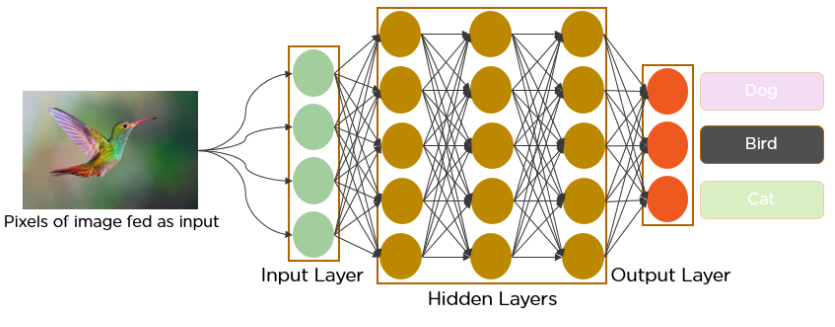
\includegraphics[width=\linewidth]{images/cnn.png}
        \caption{Simple representation of CNN}
        \label{fig:cnn}
    \end{figure}

CNNs are vital in computer vision tasks that includes object detection, image classification and segmentation. Modern CNNs uses Python to leverage advance techniques to extract and learn featurs from images. To train the models effectively, methos like hyperparameters, regularization and optimization techniques are crucial.


 \subsubsection{Single Input CNN Models}
 Deepfake detection on images, videos, or other form of media mostly uses traditional single input CNN that extract features from images using convolutional layers, pooling and fully connected layers for image classification.
 \begin{figure}[htbp]
    \centering
    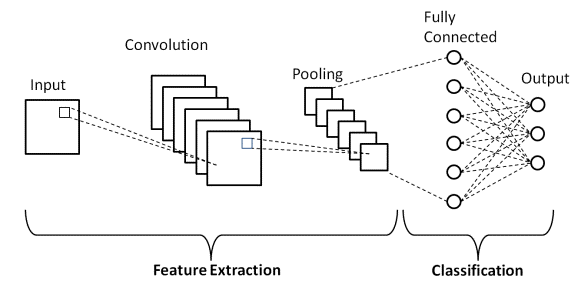
\includegraphics[width=\linewidth]{images/cnn-architecture.png}
    \caption{Single input CNN architecture}
    \label{fig:cnn-architecture}
\end{figure}

Fig. \ref{fig:cnn-architecture} depicts the main parts of CNN architecture that are stacked to generate output.


\subsubsection{Dual Input CNN Models}
DICNN (Dual Input Convolutional Neural Network) is based on base model of CNN. From numerous inputs it can update the parameters adaptively and identify deep patterns. 

\par In the base research paper \cite{Bhandari2023} referred, two input layers of size (224 x 224 x 3) were defined. The researcher processed one branch to continue with single convolution layer whose output was then flattened to concatenate flattened results of another branch. Two dense layers and dropout layers were added on top of that.
The integration of DICNN-XAI to augur fake face images and SHAP based explanation is depicted in the \ref*{fig:proposed-dicnn}. To explore blackbox approach of DICNN, after analysis it was fed to SHAP, an explainable AI.
The research was carried out from the dataset of fake and real face images from Kaggle. The dataset was divided into training, validation and testing sets. The model was trained on training set and validated on validation set. The model was tested on testing set and the results were evaluated using accuracy, F1-score, precision and recall. The results were compared with other models and the proposed model achieved better results.
\begin{figure}[htbp]
    \centering
    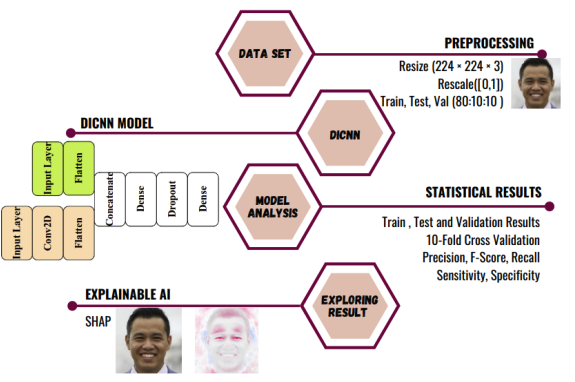
\includegraphics[width=\linewidth]{images/proposed-dicnn.png}
    \caption{Proposed DICNN model}
    \label{fig:proposed-dicnn}
\end{figure}

The model was developed in python using Keras and TensorFlow framework and the summary details for proposed DICNN architecture is depicted in \ref{tab:proposed-dicnn-model}.
 
\begin{figure}
    \centering
    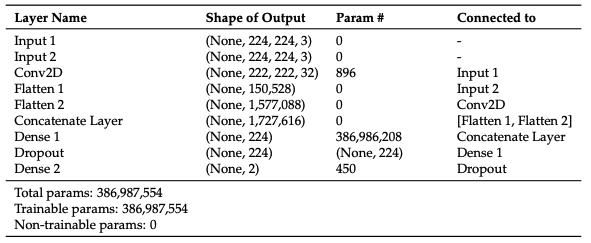
\includegraphics[width=\linewidth]{images/model-reference.png}
    \caption{Summary details for DICNN model}
    \label{fig:model-reference}
\end{figure}

\noindent Here, the researcher used the model and for evaluation, training accuracy, training loss, validation accuracy, validation loss, test accuracy, test loss, F1-score were used. The DICNN achieved average training accuracy of \(99.36 \pm 0.62\%\) and average validation accuracy of \(99.30 \pm 0.94\%\) as illustrated in the \ref{fig:dicnn-accuracy}.

\begin{figure}[htbp]
    \centering
    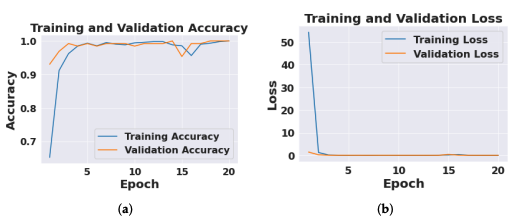
\includegraphics[width=\linewidth]{images/dicnn-accuracy.png}
    \caption{DICNN accuracy}
    \label{fig:dicnn-accuracy}
\end{figure}

\subsection{Explainable AI (XAI)}
Deep learning algorithms are blackbox in nautre and it is difficult to understand the decision making process. XAI (Explainable AI) is a field of AI that focuses on making decisions of AI models interpretable. It is crucial to understand the decision making process of AI models. So, to increase the readability and interpretability of AI models, XAI is used, especiallly in image processing \cite{Bhandari2022}, computer vision, forensics \cite{Hall2022} and criminal investigation \cite{BachmaierWinter2022}.

\subsubsection{SHAP}
SHAP (SHapley Additive exPlanations) is a method that uses game theory to explain the output of any machine learning model. It is used to explain the output of the model by computing the contribution of each feature to the prediction. \cite{SHAP}
How each pixel in the image contributes to the prediction is explained by SHAP. The SHAP values are calculated by taking the difference between the prediction of the model with the feature and without the feature. The SHAP values are then used to explain the prediction of the model.
Red color pixels contribute to prediction of class while blue pixels make class predictions less likely correct. \cite{Lundberg2017}

\par Shapley values are computed using Equation \ref{eq:shapley}
\begin{equation}
    \phi_i = \sum_{S \subseteq N \setminus \{i\}} \frac{|S|!(M - |S| - 1)!}{M!} \left[ f_x(S \cup \{i\}) - f_x(S) \right]
    \label{eq:shapley}
    \end{equation}
    
    For a particular attribute $i$, $f_x$ is the switch of results subsumed by values from SHAP. $S$ is the member of all features from feature N, with the deviation of feature $i$. The weighting factor $\frac{|S|!(M - |S| - 1)!}{M!}$ sums up the numerous ways, and the subset $S$ can be permuted. For the attributes with subset $S$, the results are denoted by $f_x(S)$ and are a result of Equation \ref{eq:fx}.
    
    \begin{equation}
    f_x(S) = \mathbb{E}[f(x) | x_S]
    \label{eq:fx}
    \end{equation}
    
    With each original trait replaced, $(x_i)$, SHAP replaces a binary variable $(z_i')$ that represents whether $x_i$ is absent or present as per Equation \ref{eq:g}.
    
    \begin{equation}
    g(z') = \phi_0 + \sum_{i=1}^{M} \phi_i z_i' = \text{bias} + \sum \text{featureContribution}
    \label{eq:g}
    \end{equation}
    
    In Equation \ref{eq:g}, for model $f(x)$, the confined surrogate model is $g(z')$.
    
\begin{figure}[htbp]
    \centering
    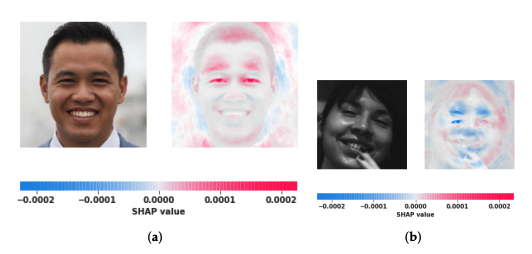
\includegraphics[width=\linewidth]{images/shap.png}
    \caption{SHAP results for (a) fake image and (b) real image}
    \label{fig:shap}
\end{figure}

As showin in Fig. \ref{fig:shap}, SHAP results for fake and real images are depicted. The red pixels intensity on fake image is high, where as on real image, the blue pixels intensity is high. The SHAP values are calculated for each pixel in the image and the results are shown in the image.


\end{section}

\pagebreak